\documentclass[tikz,border=10pt]{standalone}
\begin{document}
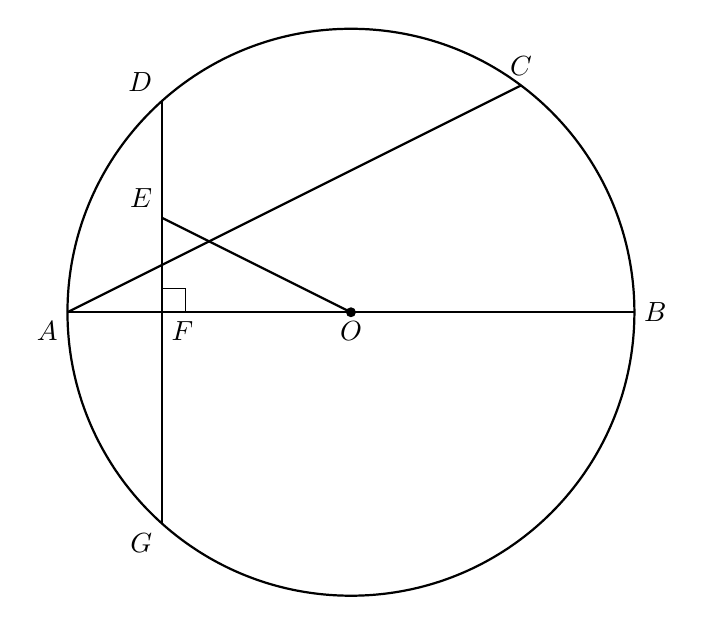
\begin{tikzpicture}[scale=1.2]
\coordinate (O) at (0,0);
\coordinate (A) at (-3,0);
\coordinate (B) at (3,0);
\coordinate (D) at (-2,2.236);
\coordinate (G) at (-2,-2.236);
\coordinate (F) at (-2,0);
\coordinate (E) at (-2,1);
\coordinate (C) at (1.8,2.4);

\draw[thick] (O) circle (3);
\draw[thick] (A) -- (B);
\draw[thick] (D) -- (G);
\draw[thick] (A) -- (C);
\draw[thick] (E) -- (O);
\draw (-2,0.25) -- (-1.75,0.25) -- (-1.75,0);

\fill (O) circle (1.5pt);

\node[below left] at (A) {$A$};
\node[right] at (B) {$B$};
\node[above] at (C) {$C$};
\node[above left] at (D) {$D$};
\node[below left] at (G) {$G$};
\node[above left] at (E) {$E$};
\node[below] at (O) {$O$};
\node[below right] at (F) {$F$};
\end{tikzpicture}
\end{document}
